\documentclass{prova}

\usepackage{amsmath}
\usepackage{amsfonts}

\setlength{\textheight}{25cm}
\setlength{\topmargin}{-1.5cm}

\renewcommand{\sin}{\,\mbox{sen}\,}
\newcommand{\ds}{\displaystyle}

\professor{Prof.\@ Adriano Barbosa}
\disciplina{C\'alculo Diferencial e Integral II}
\avaliacao{P2 2ª chamada}
\curso{Engenharia Civil}
\data{14/04/2023}

\begin{document}
	\cabecalho{5}  % o numero 5 indica a qnt de quadros na tabela de nota

    \textbf{Todas as respostas devem ser justificadas.}

    \begin{questionario}
        \q{Avalie a integral}
            \[\int_0^1 \frac{1}{1-3x}\ dx\]
        \q{Calcule a integral abaixo utilizando as substitui\c{c}\~oes indicadas:}
            \[\int \frac{\sin{x}}{\cos^3{x}}\ dx\]
            \begin{questionario}
                \qq{$\ds u=\frac{1}{\cos{x}}$.}
                \qq{$\ds u=\frac{\sin{x}}{\cos{x}}$.}
                \qq{As respostas s\~ao iguais? Explique.}
            \end{questionario}
        \q{Calcule a integral indefinida}
            \[\int \frac{x^2+x-9}{(x-3)(x-1)^2}\ dx\]
        \q{Calcule a \'area da regi\~ao delimitada pelas curvas $x=0$, $x=1$, $y=0$
            e $y=x\sin{(2x)}$.}
            \begin{figure}[h]
                \centering
                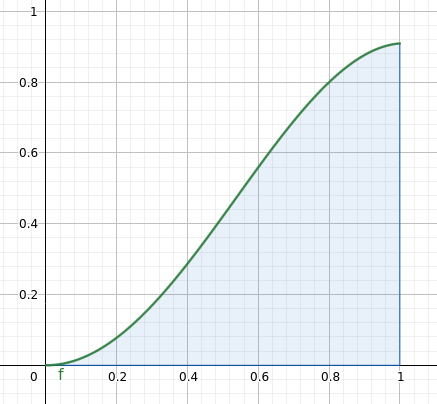
\includegraphics[width=0.3\textwidth]{area.png}
            \end{figure}
        \q{Determine o valor positivo de $k$ tal que}
            \[\int_{-\infty}^{0} \frac{1}{x^2+k^2}\ dx = \pi\]
    \end{questionario}
    \vspace{-1cm}
\end{document}
